\documentclass[reqno,a4paper,12pt]{amsart}

\usepackage{amsmath,amssymb,amsthm,geometry,xcolor,soul,graphicx}
\usepackage{titlesec}
\usepackage{enumerate}
\usepackage{lipsum}
\usepackage{listings}
\RequirePackage[most]{tcolorbox}
%\usepackage{braket}
\usepackage{xeCJK}
\setCJKmainfont{Kai}
\geometry{left=0.7in, right=0.7in, top=1in, bottom=1in}


\renewcommand{\baselinestretch}{1.3}

\title{固体物理第三次作业}
\author{董建宇 ~~ 2019511017}

\begin{document}

\maketitle
\titleformat{\section}[hang]{\small}{\thesection}{0.8em}{}{}
\titleformat{\subsection}[hang]{\small}{\thesubsection}{0.8em}{}{}

\section{\textbf{(4.1) Fermi Surface in the Free Electron (Sommerfeld) Theory of Metals}}
\begin{enumerate}[(a)]
	\item Explain what is meant by the Fermi energy, Fermi temperature and the Fermi surface of a metal. 
	
	\begin{tcolorbox}[breakable, colback = black!5!white, colframe = black]
	费米能量为温度为$0K$时的化学势。费米温度为费米能量对应的温度:
	\[
		T_F = \frac{E_F}{k_B}.
	\]
	费米面为在动量空间中,在温度为$0K$条件下,量子态的表面。
	\end{tcolorbox}
		
	\item Obtain an expression for the Fermi wavevector and the Fermi energy for a gas of electrons (in 3D). \\
	$\triangleright$ Show that the density of states at the Fermi surface, $dN/dE_F$ can be written as $3N/2E_F$. 
	
	\begin{tcolorbox}[breakable, colback = black!5!white, colframe = black]
	在温度为$0K$时,Fermi-Dirac分布为:
	\[
		f(\mathcal{E}) = \left\{ \begin{aligned}
			1,~ &for ~ \mathcal{E} \leq E_F; \\
			0,~ &for ~ \mathcal{E} > E_F.
		\end{aligned}\right.
	\]
	利用粒子数总和为$N$可知:
	\[
		N = V\int_0^{+\infty} g(\mathcal{E}) f(\mathcal{E})\,d\mathcal{E} = V \int_0^{E_F} \frac{(2m)^{3/2}}{2\pi^2\hbar^3}\sqrt{\mathcal{E}}\,d\mathcal{E} = V \frac{(2mE_F)^{3/2}}{3\pi^2\hbar^3}.
	\]
	其中能量$E_F$与波矢$k_F$关系为:
	\[
		E_F = \frac{\hbar^2 k_F^2}{2m}.
	\]
	带入上式可得:
	\[
		k_F = \left( \frac{3\pi^2 N}{V} \right)^{1/3}.
	\]
	同时可以计算得:
	\[
		\frac{dN}{dE_F} = V \frac{(2m)^{3/2}}{2\pi^2\hbar^3} \sqrt{E_F} = V\frac{(2mE_F)^{3/2}}{3\pi^2\hbar^3}\frac{3}{2E_F} = \frac{3}{2}\frac{N}{E_F}.
	\]
	\end{tcolorbox}
	
	\item Estimate the value of $E_F$ for a sodium [The density of sodium atoms is roughly $1~gram/cm^3$, and sodium has atomic mass of roughly 23. You may assume that there is one free electron per sodium atom (sodium has valence one)] 
	
	\begin{tcolorbox}[breakable, colback = black!5!white, colframe = black]
	利用密度和相对原子质量表示自由电子数目$N$:
	\[
		N = \frac{m}{M}N_A = \frac{\rho VN_A}{M}.
	\]
	即
	\[
		n = \frac{N}{V} = \frac{\rho N_A}{M}.
	\]
	则费米能量为:
	\[
		E_F = \frac{(3\pi^2\hbar^3n)^{2/3}}{2m_e} = 3.215 eV.
	\]
	\end{tcolorbox}
	
	\item Now consider a two-dimensional Fermi gas. Obtain an expression for the density of states at the Fermi surface. 
	
	\begin{tcolorbox}[breakable, colback = black!5!white, colframe = black]
	对于二维费米气体有:
	\[
		N = 2\sum_{\vec{k}} \vec{k} f(\varepsilon) = \frac{2L^2}{(2\pi)^2} \int 2\pi k\,dk = \frac{S}{2\pi} \int_0^{E_F} \frac{2m}{\hbar^2} \,d\mathcal{E} = \frac{mSE_F}{\pi\hbar^2}.
	\]
	则费米面处态密度为:
	\[
		g(E_F) = \frac{\partial N}{\partial E_F}= \frac{mS}{\pi\hbar^2}.
	\]
	\end{tcolorbox}
\end{enumerate}

\section{\textbf{(4.2) Velocities in the Free Electron Theory}}
\begin{enumerate}[(a)]
	\item Assuming that the free electron theory is applicable: show that the speed $v_F$ of an electron at the Fermi surface of a metal is $v_F = \frac{\hbar}{m}(3\pi^2n)^{1/3}$ where $n$ is the density of electrons. 
	
	\begin{tcolorbox}[breakable, colback = black!5!white, colframe = black]
	由第一题可知,费米能量为:
	\[
		E_F = \frac{1}{2}mv_F^2 = \frac{(3\pi^2n)^{2/3}\hbar^2}{2m}.
	\]
	则费米速度可以解得:
	\[
		v_F = \frac{\hbar}{m}(3\pi^2n)^{1/3}.
	\]
	\end{tcolorbox}
	
	\item Show that the mean drift speed $v_d$ of an electron in an applied electric field $E$ is $v_d = \vert \sigma E/(ne) \vert$, where $\sigma$ is the electrical conductivity, and show that $\sigma$ is given in terms of the mean free path $\lambda$ of the electrons by $\sigma = ne^2\lambda/(mv_F)$.
	
	\begin{tcolorbox}[breakable, colback = black!5!white, colframe = black]
	电流密度为:
	\[
		\vec{j} = -ne\vec{v}_d = \sigma \vec{E}.
	\]
	则平均漂移速度大小为:
	\[
		v_d = \left\vert \frac{\sigma E}{ne} \right\vert.
	\]
	其中电导率为:
	\[
		\sigma = \frac{ne^2\tau}{m}.
	\]
	利用平均自由程$\lambda = v_F\tau$,有:
	\[
		\sigma = \frac{ne^2\lambda}{mv_F}.
	\]
	\end{tcolorbox}
	
	\item Assuming that the free electron theory is applicable to copper: 
	\begin{enumerate}[(i)]
		\item calculate the values of both $v_d$ and $v_F$ for copper at 300K in an electric field of $1 V/m$ and comment on their relative magnitudes. 
		\begin{tcolorbox}[breakable, colback = black!5!white, colframe = black]
		漂移速度为:
		\[
			v_d = \frac{\sigma E}{ne} \approx 4.36 \times 10^{-3}m/s.
		\]
		约为2倍蜗牛爬行速度。(very very slow) \\
		由于300K远小于费米温度,费米速度近似为:
		\[
			v_F = \frac{\hbar}{m}(3\pi^2n)^{1/3} \approx 1.57 \times 10^{6} m/s.
		\]
		约为$0.5\%$倍的光速。(pretty fast)
		\end{tcolorbox}
		
		\item estimate $\lambda$ for copper at 300K and comment upon its value compared to the mean spacing between the copper atoms.
		\begin{tcolorbox}[breakable, colback = black!5!white, colframe = black]
		利用电导率可估计平均自由程为:
		\[
			\lambda = \frac{mv_F\sigma}{ne^2} \approx 3.89 \times 10^{-8} m.
		\]
		铜原子晶格常数约为$d = 3.6\times 10^{-10}m$,则平均自由程约为108个铜原子直径。
		\end{tcolorbox}
	\end{enumerate}
\end{enumerate}

\section{\textbf{(4.5) Chemical Potential of 2D Electrons}}
\begin{enumerate}[(a)]
	\item Show that for free electron gas in two dimensions, the chemical potential $\mu$ is independent of the temperature so long as $T<<\mu$. Hint: first examine the density of states in two dimensions. 
	\begin{tcolorbox}[breakable, colback = black!5!white, colframe = black]
	由第一题可知,二维自由电子气的态密度为:
	\[
		g(\mathcal{E}) = \frac{mS}{\pi\hbar^2} = g_0.
	\]
	则化学式由下式给出:
	\[
		n = \int_0^{+\infty} \,dE g_0\frac{1}{e^{\beta(E-\mu)}+1}
	\]
	令$x = E-\mu$, $y = e^{-\beta x}$,则积分化为:
	\[
		n = g_0 \int_{-\mu}^{+\infty} \frac{e^{-\beta x}}{e^{-\beta x} + 1} = \frac{g_0}{\beta}\int_0^{e^{\beta\mu}}\,dy \frac{1}{y+1} = \frac{g_0}{\beta}\ln(e^{\beta\mu}+1).
	\]
	当$\beta\mu$很大时,有:
	\[
		n = g_0\mu + \mathcal{O}(e^{-\beta\mu}).
	\]
	即当$k_BT<<\mu$,化学式$\mu$与温度无关。
	\end{tcolorbox}
\end{enumerate}

\section{\textbf{(4.6) Chemical Potential at T = 0}}
\begin{enumerate}[(a)]
	\item Consider a system of $N$ non-interacting electrons. At $T = 0$ the $N$ lowest-energy eigenstates will be filled and all the higher energy eigenstates will be empty. Show that at $T=0$ the energy of the chemical potential is precisely half way between the highest energy energy filled eigenstate and the lowest-energy unfilled eigenstate. 
	\begin{tcolorbox}[breakable, colback = black!5!white, colframe = black]
	由于费米温度远大于0,远离费米面的内层电子几乎不会受温度扰动的影响,所以只需考虑费米面附近的电子态。令最高填充态能级能量为$E_1$,简并度为$g_1$;最低未填充态能级能量为$E_2$,简并度为$g_2$。电子总数守恒有:
	\[
		g_1 = \frac{g_1}{e^{\beta(E_1-\mu)}+1} + \frac{g_2}{e^{\beta(E_2-\mu)}+1}.
	\]
	令$x = e^{\beta(E_1-\mu)}$, $y = e^{\beta(E_1-E_2)}$,则方程可化为:
	\[
		g_1x^2 + (g_1-g_2)z x - g_2z = 0.
	\]
	可以解得$(x>0,z\to 0)$:
	\[
		x = \frac{(g_2-g_1)z + \sqrt{(g_1-g_2)^2z^2+4g_1g_2z}}{2g_1} \approx \sqrt{\frac{g_2}{g_1}z}.
	\]
	两侧取对数可得:
	\[
		\beta(E_1-\mu) = \frac{1}{2}(\ln g_2 - \ln g_1 + \beta(E_1-E_2)).
	\]
	当$T\to 0$时,有$\beta\to\infty$,则上式为:
	\[
		\lim_{\beta\to\infty}\mu = \frac{E_1+E_2}{2}.
	\]
	\end{tcolorbox}
\end{enumerate}

\section{\textbf{(4.7) More Thermodynamics of Free Electrons}}
\begin{enumerate}[(a)]
	\item Show that the kinetic energy of a free electron gas in three dimensions is $E = \frac{3}{5}E_FN$.
	\begin{tcolorbox}[breakable, colback = black!5!white, colframe = black]
	态密度为:
	\[
		g(\mathcal{E}) = \frac{(2m)^{3/2}}{2\pi^2\hbar^3}\sqrt{\mathcal{E}}.
	\]
	则可以计算粒子数与能量如下:
	\[
		N = V\int_0^{E_F} \,d\mathcal{E}g(\mathcal{E}) = \frac{(2m)^{3/2}V}{2\pi^2\hbar^3} \frac{2}{3} E_F^{3/2}.
	\]
	\[
		E = V\int_0^{E_F} \,d\mathcal{E}g(\mathcal{E}) \mathcal{E} = \frac{(2m)^{3/2}V}{2\pi^2\hbar^3} \frac{2}{5} E_F^{5/2}.
	\]
	则在三维自由电子气中,动能为:
	\[
		E = \frac{3}{5}E_FN.
	\]
	\end{tcolorbox}
	
	\item Calculate the pressure $P = -\partial E/\partial V$, and then the bulk modulus $B = -V\partial P/\partial V$.
	\begin{tcolorbox}[breakable, colback = black!5!white, colframe = black]
	由第一题可知:
	\[
		E_F = \frac{1}{2m}\left( \frac{3\pi^2\hbar^3N}{V} \right)^{2/3}.
	\]
	则有:
	\[
		E = \frac{3(3\pi^2\hbar^3)^{2/3}N^{5/3}}{10m} V^{-2/3}.
	\]
	则压强为:
	\[
		P = -\frac{\partial E}{\partial V} = \frac{3(3\pi^2\hbar^3)^{2/3}N^{5/3}}{10m} \frac{2}{3} V^{-5/3} = \frac{2E}{3V} = \frac{2E_FN}{5V}.
	\]
	体弹性模量为:
	\[
		B = -V\frac{\partial P}{\partial V} = \frac{5P}{3} = \frac{2E_FN}{3V}.
	\]
	\end{tcolorbox}
	
	\item Given that the density of atoms in sodium is $2.53\times 10^{22}cm^{-3}$ and that of potassium is $1.33\times 10^{22}cm^{-3}$, and given that both of these metals are monovalent (i.e., have one free electron per atom), calculate the bulk modulus associated with the electrons in these materials. Compare your results to the measured values of $6.3$ $GPa$ and $3.1$ $GPa$ respectively.
	\begin{tcolorbox}[breakable, colback = black!5!white, colframe = black]
	费米能量为:
	\[
		E_F = \frac{1}{2m}(3\pi^2\hbar^3n)^{2/3}.
	\]
	则体弹性模量为:
	\[
		B = \frac{1}{3m}(3\pi^2\hbar^3)^{2/3}n^{5/3}.
	\]
	代入数据可得:
	\[
		B_{Na} = 8.49\times 10^{9}Pa, ~ B_{K} = 2.91 \times 10^{9} Pa.
	\]
	\end{tcolorbox}
\end{enumerate}

\section{\textbf{拟合Nb2P5费米温度}}
\begin{enumerate}[(a)]
	\item 绘制热熔除以温度随温度平方变化的直线拟合(假设价电子数目为1)。
	\[
		\frac{C}{T} = \frac{\pi^2R}{2T_F} + \frac{12\pi^4R}{5}\frac{T^2}{T_D^3}.
	\]
	\begin{center}
		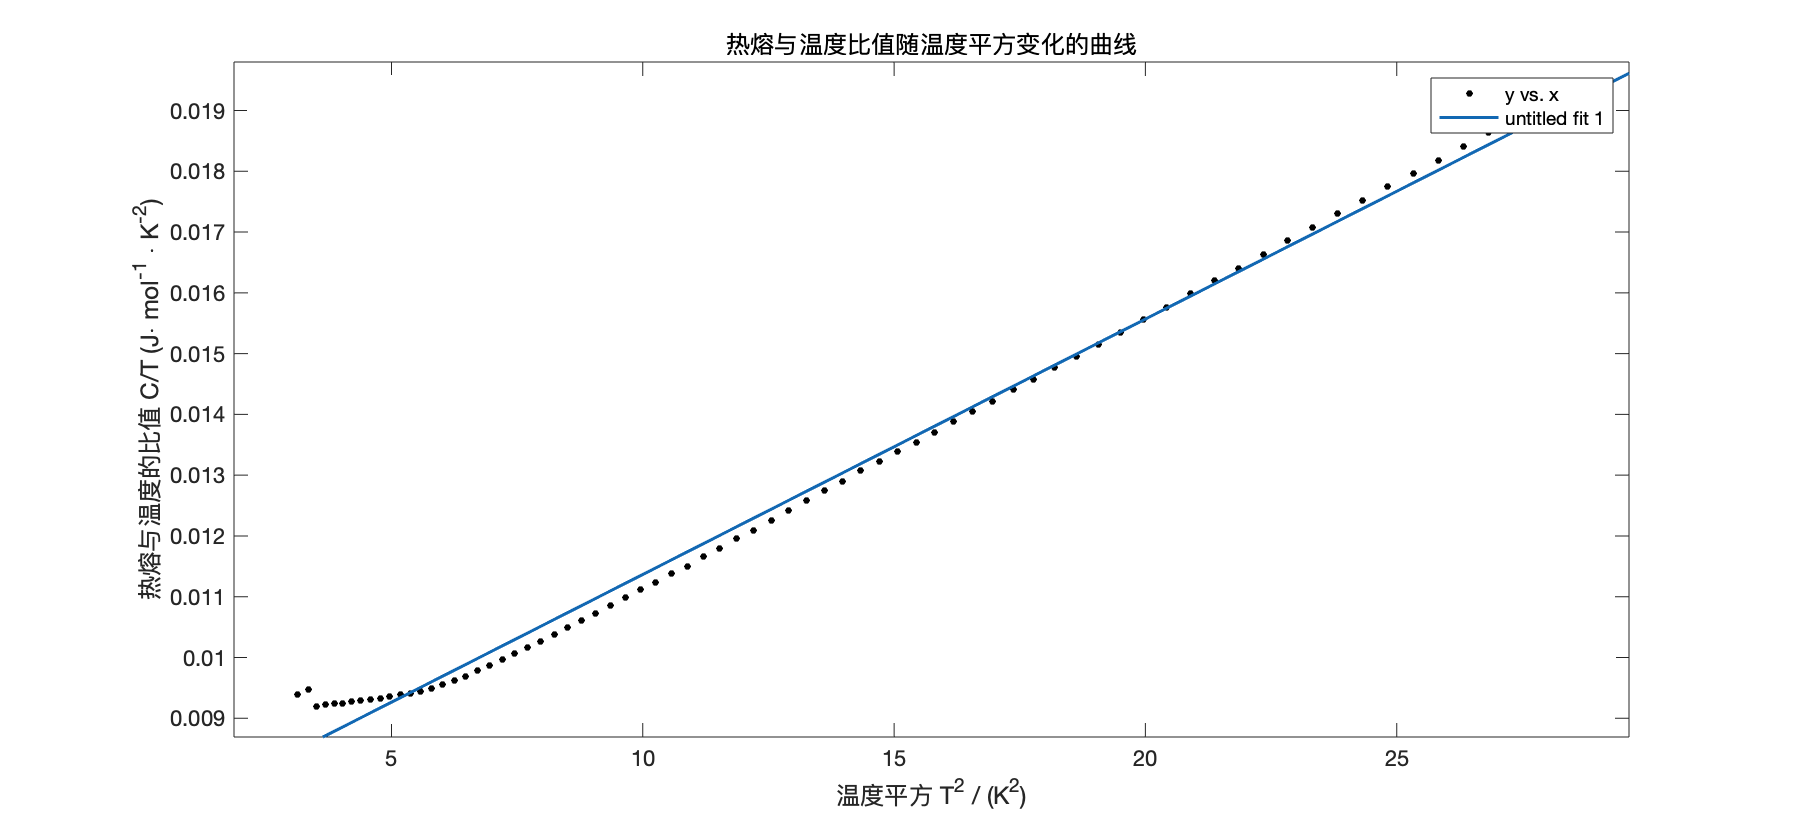
\includegraphics[scale = 0.28]{Nb2P5.png}
	\end{center}
	拟合直线方程如下$(R^2 = 0.9938)$:
	\begin{center}
		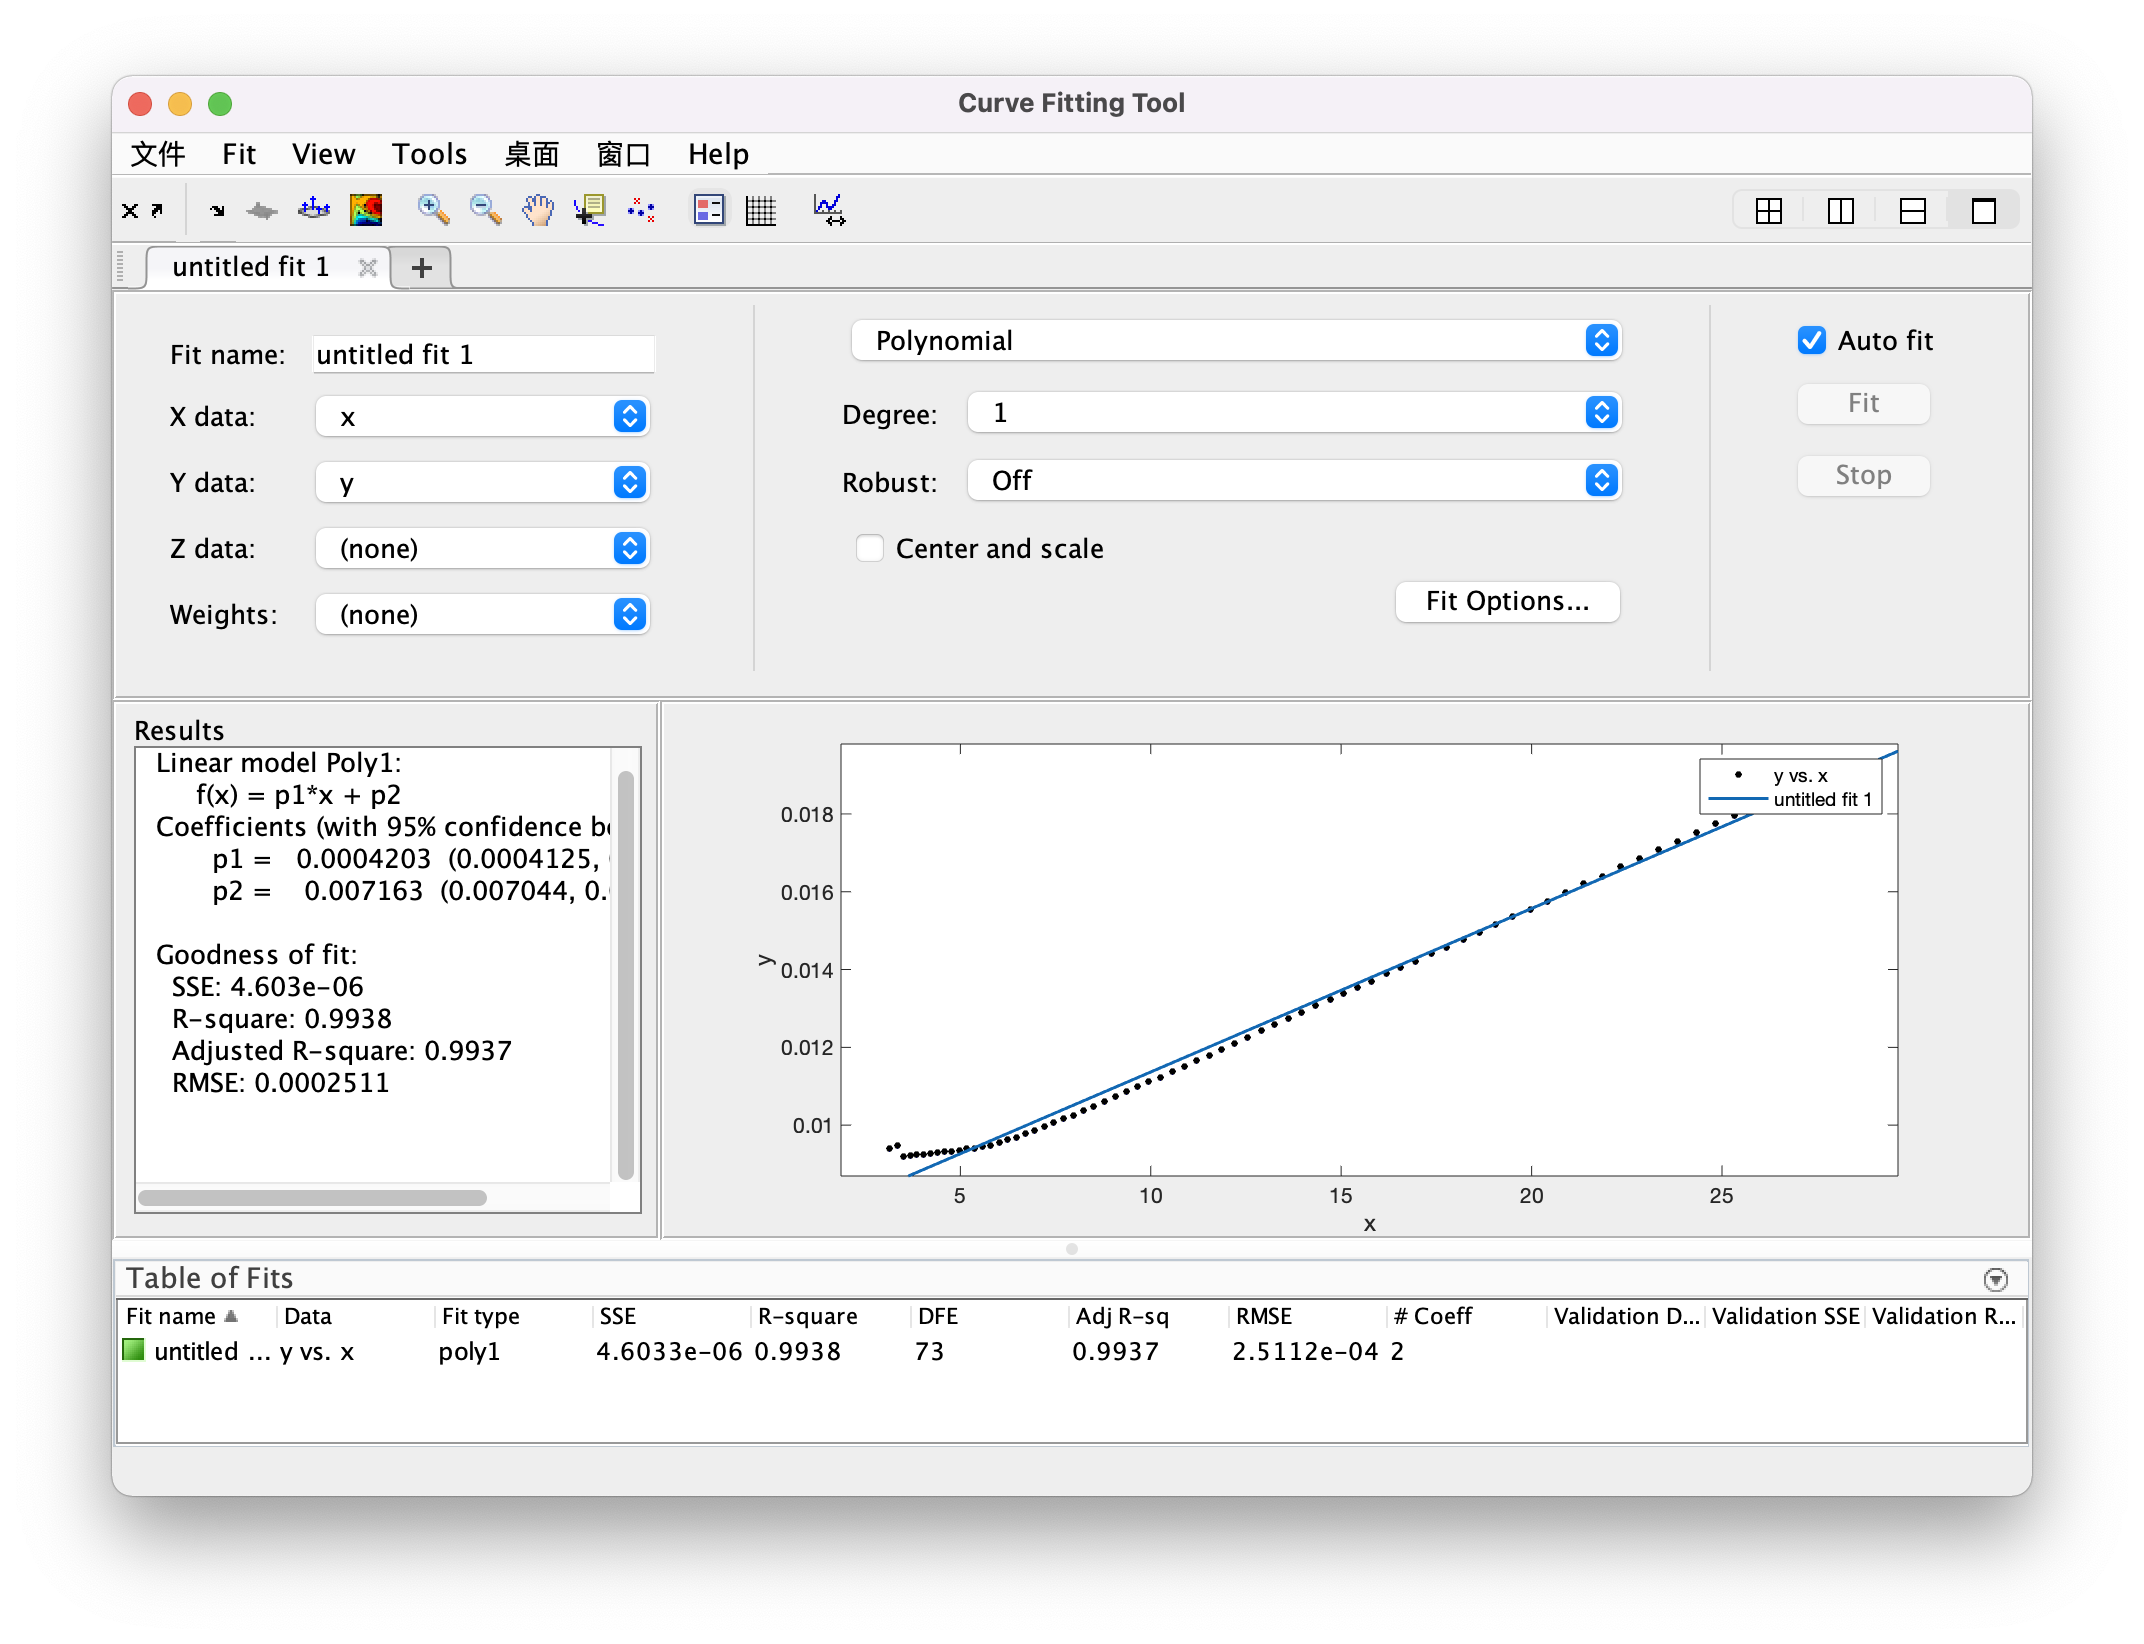
\includegraphics[scale = 0.36]{data.png}
	\end{center}

	\item 读取零阶项系数为$0.007163~J \cdot mol^{-1} \cdot K^{-2}$。则有:
	\[
		\frac{\pi^2N_Ak_B}{2T_F} = 0.007163~J \cdot mol^{-1} \cdot K^{-2}.
	\]
	可以计算得费米温度约为:
	\[
		T_F \approx 5725K.
	\]
\end{enumerate}



\end{document}